\textbf{Onderbouw je antwoorden altijd door beredenering en/of berekening.}

Gegeven is een synchrone driefasen motor met een permanent magneet rotor die wordt aangestuurd met een frequentieregelaar. Het aandrijfsysteem (motor en regelaar) is ontworpen op een nominale spanning van 400V/100Hz. Bij een instelling van de frequentieregelaar op 60 Hz heeft de motor de onderstaande
koppel-toerenkarakteristiek.

\begin{figure}[h]
    \centering
    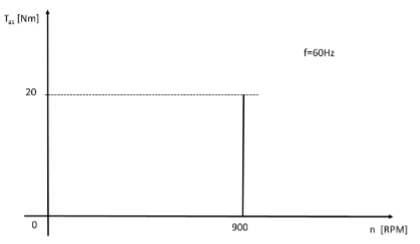
\includegraphics[scale=1.5]{3-uitleg.png}
\end{figure}

\begin{enumerate}
    \item [a.] \textbf{Bepaal de polen van deze motor}
    
        Poolparen:
        $ P = \frac{60 \times f}{n_{s}} = \frac{60 \times 60}{900} = 4 poolparen = 8 polen$

    \item [b.] \textbf{Bepaal de lasthoek van de motor bij een lastkoppel van 10 Nm.}
    
        $ \delta = 90 \times \frac{T_{last}}{T_{max}} = 90 \times \frac{10}{20} = 45 graden$

\end{enumerate}

De motor wordt gebruikt om een last aan te drijven waarvan de koppel-toerenkarakteristiek tijdens bedrijf kan variëren in het rode gebied dat is aangegeven in onderstaand figuur.
\begin{figure}[h]
    \centering
    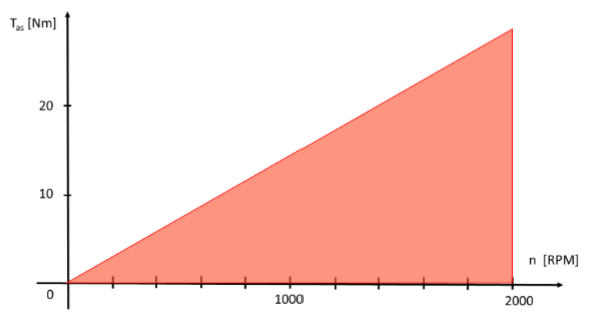
\includegraphics[scale=1]{3b-uitleg.png}
\end{figure}

\begin{enumerate}
    \item [c.] \textbf{Wat is het maximale koppel en toerental van het aandrijfsysteem (motor en regelaar) zodat voldaan wordt aan de eis dat het toerental constant blijft?}
    
        $rpm_{max} = \frac{f \times 60}{p} = \frac{100 \times 60}{4} = 1500rpm$

        Omdat je koppel toerenkarakteristiek over de horizontale as verschuift omdat je rpm meer wordt blijft je koppel gelijk. ofterwijl 20Nm.


    \item [d.] \textbf{Bepaal het maximale vermogen dat de motor op de last kan overbrengen bij een lastkoppel van 10 Nm.}     
    
        $ P_{uit} = \omega_{s} \times T_{em} = 157 \times 10 = 1570 Watt $

        $ \omega_{s} 
        = \frac{2 \times \pi \times rpm}{60} 
        = \frac{2 \times \pi \times 1500}{60} 
        = 157 rad/s$

    \item [e.] \textbf{Wat is het maximale toerental van de motor waarmee een constante last van 20 Nm aangedreven kan worden?}
    
        1500rpm is het macimale toerental van de motor waarmee een last van 20Nm aangedreven kan worden.\\
        Zie ook opgave c en d.

\end{enumerate}